\documentclass{techbrief}

\usepackage{tikz}
\usetikzlibrary{shapes.geometric, calc}
\usepackage{cancel}

\title{Relationship between formulations of classical mechanics}
\author{Matteo Carcassi}
\category{Classical mechanics}
\tags{Newtonian mechanics, Lagrangian mechanics, Hamiltonian mechanics}

\begin{document}
	
	\maketitle
	
	\begin{abstract}
		We show that the three formulations of classical mechanics are inequivalent: not all Newtonian systems are Hamiltonian systems and vice-versa, while Lagrangin systems are exactly those that are Hamiltonian and Newtonian.
	\end{abstract}
	
	\section{Introduction}
	While it is often stated that the three formulations in classical mechanics, Newtonian, Lagrangian, and Hamiltonian, are equivalent, there are systems that can be described in one formulation but not another. In this note, we show Newtonian and Hamiltonian mechanics can apply to different systems while Lagrangian mechanics applies on the intersection of the other two.
	
	\section{Conditions}
		\begin{condition}[Newtonian Mechanics]{NM}
			The state of the system is described by position $x^{i}$ and velocity $v^{i}$. The dynamics is specified by forces $F^{i}(x^{j},v^{k},t)$ which are locally Lipschitz continuous. The evolution of the system over time $t$ is given by Newton's second law $F^{i} = d_{t}(mv^{i})$ where $m$ is the mass of the system.
		\end{condition}
		
		\begin{condition}[Hamiltonian Mechanics]{HM}
			The state of the system is described by position $q^{i}$ and conjugate momentum $p_{i}$. The dynamics is specified by a Hamiltonian $H(q^{i},p_{j},t)$ which is differentiable and whose derivatives are at least Lipschitz continuous. The evolution of the system over time $t$ is given by Hamilton's equations $d_{t}q^{i} = \partial_{p_{i}}H$ and $d_{t}p_{i} = -\partial_{q^{i}}H$.
		\end{condition}
		
		\begin{condition}[Lagrangian Mechanics]{LM}
			The state of the system is described by position $x^{i}$ and velocity $v^{i}$. The dynamics is specified by a Lagrangian $L(x^{i},v^{j},t)$ with the property that the Hessian matrix $\partial_{v^{i}}\partial_{v^{j}}L$ is invertible (i.e. hyperregularity). The evolution of the system over time $t$ is given by the Euler-Lagrange equations $\partial_{x^{i}}L = d_{t}\partial_{v^{i}}L$.
		\end{condition}
	
	\section{Theorems}
	\begin{thrm}
		Condition \ref{LM} is equivalent to \ref{NM} and \ref{HM}.
	\end{thrm}
	\begin{proof}
		We first show that \ref{LM} implies \ref{NM}. Let $m$ be the mass of the system. We have $d_{t}v^{i}=a^{i}=\frac{F^i}{m}$. From the Euler-Lagrange equations, we have:
		\begin{equation}
			\begin{aligned}
				\partial_{x^i}L&= d_t \partial_{v^i} L = \partial_{x^j} \partial_{v^i} L d_t x^j + \partial_{v^k} \partial_{v^i} L \, d_t v^k \\ &= \partial_{x^j} \partial_{v^i} L \, v^j + \partial_{v^k} \partial_{v^i} L \, a^k \\
				\partial_{v^k} \partial_{v^i} L \, a^k &= \partial_{x^i}L - \partial_{x^j} \partial_{v^i} L \, v^j .
			\end{aligned}
		\end{equation} 
		Since the Hessian matrix $\partial_{v^{i}}\partial_{v^{j}}L$ is invertible, we have
		\begin{equation}
			\begin{aligned}
				F^i &= m a^i = m (\partial_{v^k} \partial_{v^i} L)^{-1}(\partial_{x^i}L - \partial_{x^j} \partial_{v^i} L \, v^j).
			\end{aligned}
		\end{equation} 
		
		
		We now show that \ref{LM} implies \ref{HM}. We define the state variables and the Hamiltonian for the Hamiltonian system to be
		\begin{equation}
			\begin{aligned}
				q^{i} &= x^{i} \\
				p_{i} &= \partial_{v^{i}}L \\
				H &= v^{i} p_{i} - L
			\end{aligned}
		\end{equation}
		From the Euler-Lagrange equations:
		\begin{equation}
			\begin{aligned}
				\partial_{x^{i}}L = d_{t}\partial_{v^{i}}L = d_{t}p_{i}
			\end{aligned}
		\end{equation}
		And by performing a total differentiation of the Hamiltonian:
		\begin{equation}
			\begin{aligned}
				dH &= p_{i}dv + v^{i}dp - (\partial_{x^{i}}Ldx + \partial_{v^{i}}Ldv + \partial_{t}Ldt) \\
				&= p_{i}dv + v^{i}dp - (d_{t}p_{i}dq + p_{i}dv + \partial_{t}Ldt) \\
				&= -d_{t}p_{i}dq + d_{t}q^{i}dp - \partial_{t}Ldt \\
				&= \partial_{q^{i}}Hdq + \partial_{p_{i}}Hdp + \partial_{t}Hdt
			\end{aligned}
		\end{equation}
		By matching the components of the total derivative, we recover Hamilton's equations:
		\begin{equation}
			\begin{aligned}
				d_{t}q^{i} = \partial_{p_{i}}H \\
				d_{t}p_{i} = -\partial_{q^{i}}H
			\end{aligned}
		\end{equation}
		
		Now to show the converse. In order for both \ref{NM} and \ref{HM} to be true, there must exist a map between the states $(x^{i},v^{j},t)$ and $(q^{i},p_{j},t)$. Hamilton's equation gives a way to relate velocity and conjugate momentum:
		\begin{equation}
			\begin{aligned}
				v^{i} = d_{t}q^{i} = \partial_{p_{i}}H
			\end{aligned}
		\end{equation}
		Then from Hamilton's equations, we can recover the Euler-Lagrange equations:
		\begin{equation}
			\begin{aligned}
				-\partial_{q^{i}}H &= d_{t}p_{i} = d_{t}\partial_{v^{i}}L \\
				-\partial_{q^{i}}H &= - \partial_{q^{i}}(pv) + \partial_{q^{i}}L\\
				&= - (\partial_{q^{i}}p_{i}) v^{i} - \cancel{(\partial_{q^{i}}v^{i}) p_{i}} + \partial_{p^{i}}H\partial_{q^{i}}p_{i} + \partial_{q^{i}}L \\
				&= \partial_{q^{i}}p_{i}(\partial_{p_{i}}H - v) + \partial_{q^{i}}L \\
				&= \partial_{x^{i}}L = d_{t}\partial_{v^{i}}L
			\end{aligned}
		\end{equation}
	\end{proof}
	\begin{thrm}
		Conditions \ref{NM} and \ref{HM} are independent
	\end{thrm}
	\begin{proof}
	We first show that \ref{NM} does not imply \ref{HM}. Note that the dynamics in \ref{NM} is specified by multiple independently chosen force functions while in \ref{HM} is specified by a single Hamiltonian function. Since a continuous surjective map from the space of a single function to multiple functions does not exist, there exists at least a system that can be described by \ref{NM} that cannot be described by \ref{HM}. \\

	We now show that \ref{HM} does not imply \ref{NM} by giving a counter-example. Consider the photon as a classical particle. We can write the Hamiltonian by expressing the energy as a function of momentum
	\begin{equation}
		H=\hbar | \omega| = c \hbar |k| = c |p|.
	\end{equation}
	We find the evolution of the particle to be
	\begin{equation}
		\begin{aligned}
			d_t q^i &= c \frac{p^i}{|p|} \\
			d_t p_i &= 0.
		\end{aligned}
	\end{equation} 
	The speed of the photon is the constant $c$, and therefore the momentum cannot be reconstructed from the velocity. This means that the state of the system cannot be described by position and velocity, violating condition \ref{NM}.
	
	Since there exist systems that can be described by both Newtonian and Hamiltonian mechanics, \ref{NM} and \ref{HM} are compatible in the sense that they can be true at the same time. Conversely, the existence of quantum systems provide a case in which \ref{NM} and \ref{HM} are false. This means that the truth of one condition does not depend on the truth of the other condition, and therefore \ref{NM} and \ref{HM} are independent.
	\end{proof}
	
	\begin{figure}[h]
		\centering
		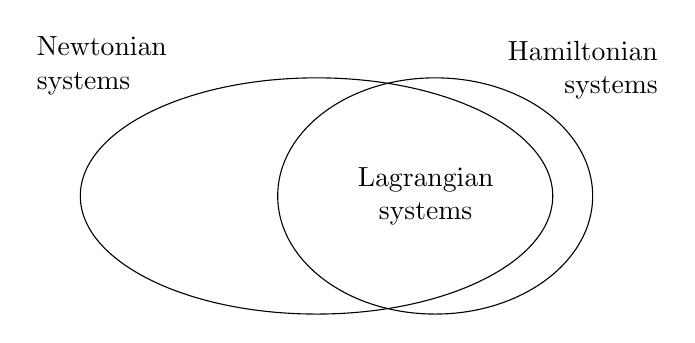
\begin{tikzpicture}
			\node[ellipse, minimum width=6cm, minimum height=3cm, draw, left] (ns){};
			\node [align=left, above] at ([xshift=-6mm,yshift=1mm]ns.north west) {Newtonian \\systems};
			
			\node[ellipse, minimum width=4cm, minimum height=3cm, draw] (hs) at ([xshift=-1.5cm]ns.east){};
			\node [align=right, above right] at ([xshift=8mm, yshift=-4mm]hs.north) {Hamiltonian\\ systems};
			\node [align=center, right] at ([xshift=9
			mm]hs.west) {Lagrangian \\systems};
		\end{tikzpicture}
		\caption {Not all Hamiltonian systems are Newtonian and not all Newtonian systems are Hamiltonian. All Lagrangian systems are both Newtonian and Hamiltonian.}\label{rp-cm-fig-vennDiagramEarly}
	\end{figure}
	\section{Conclusion}
		We have found a more precise relationship between the three formulations of classical mechanics. The realm of applicability of the different formulation can also be characterized in terms of physical assumptions within the larger work of Reverse Physics.
	
\end{document}